Gibt es einen Zusammenhang zwischen Einkommen $X$ und Glück?
Ein Forscher führt dazu eine Befragung durch, in der Teilnehmer
ihr Einkommen in kCHF und eine numerische Note $G$ zwischen 1 und 
10 zur Bewertung ihres ``Glücks'' angeben müssen.
Ein kleiner Ausschnitt aus den erhobenen Daten ist in der folgenden
Tabelle wiedergegeben:
\begin{center}
\begin{tabular}{|>{$}c<{$}|>{$}r<{$}|>{$}r<{$}|}
\hline
i&\text{Einkommen [kCHF]}&\text{``Glück''}\\
\hline
1&15&3\\
2&20&4\\
3&30&5\\
4&50&7\\
5&75&9\\
\hline
\end{tabular}
\end{center}

\begin{teilaufgaben}
\item Gibt es einen einfachen Zusammenhang zwischen $X$ und $G$?
\item Beurteilen Sie die Qualität Ihres Modells.
\item Wie glücklich müsste nach dieser Skala Amazon-Chef Jeff Bezos
sein mit einem Jahreslohn von ca.~$\text{CHF}\,311\cdot 10^6$
(gemäss {\tiny\url{https://k.at/entertainment/so-viel-geld-verdient-jeff-bezos-in-einer-sekunde/400966784}}).
\end{teilaufgaben}

\ifthenelse{\boolean{loesungen}}{
\begin{figure}
\centering
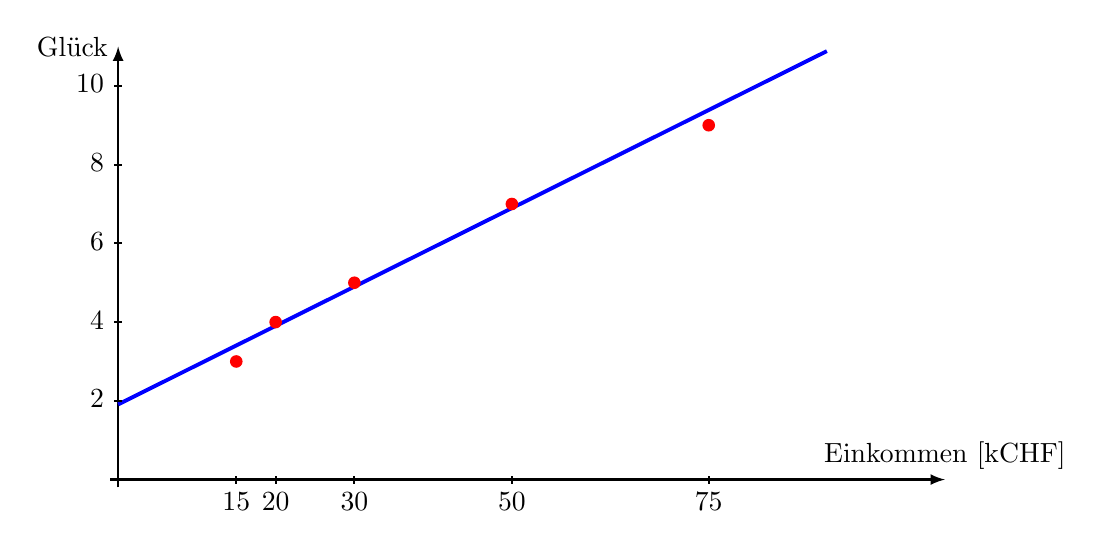
\begin{tikzpicture}[>=latex,thick]
\draw[->] (-0.1,0) -- (10.5,0) coordinate[label={Einkommen [kCHF]}];
\draw[->] (0,-0.1) -- (0,5.5) coordinate[label={left:Glück}];
\def\punkt#1{({0.1*#1},{0.5*(0.0997*(#1)+1.9095)})}
\def\p#1#2{({0.1*#1},{0.5*#2})}
\draw[color=blue,line width=1.4pt] \punkt{0} -- \punkt{90};
\fill[color=red] \p{15}{3} circle[radius=0.08];
\fill[color=red] \p{20}{4} circle[radius=0.08];
\fill[color=red] \p{30}{5} circle[radius=0.08];
\fill[color=red] \p{50}{7} circle[radius=0.08];
\fill[color=red] \p{75}{9} circle[radius=0.08];
\def\eti#1{
	\draw ({0.1*#1},-0.05) -- ({0.1*#1},0.05);
	\node at ({0.1*#1},0) [below] {$#1\mathstrut$};
}
\eti{15}
\eti{20}
\eti{30}
\eti{50}
\eti{75}
\foreach \y in {2,4,6,8,10}{
	\draw (-0.05,{0.5*\y}) -- (0.05,{0.5*\y});
	\node at (-0.05,{0.5*\y}) [left] {$\y\mathstrut$};
}
\end{tikzpicture}
\caption{Regressionsgerade für die Daten von Aufgabe~\ref{40000049}
\label{40000049:fig}}
\end{figure}
}{}

\begin{loesung}
\begin{teilaufgaben}
\item
Ein linearer Zusammenhang zwischen $X$ und $G$ kann mit Hilfe von
linearer Regression gefunden werden.
Dazu verwenden wir die Tabelle
\begin{center}
\begin{tabular}{|>{$}c<{$}|>{$}r<{$}>{$}r<{$}|>{$}r<{$}>{$}r<{$}|>{$}r<{$}|}
\hline
i&    x_i&   g_i\phantom{.0}& x_i^2& g_i^2&x_ig_i\\
\hline
1&     15&     3\phantom{.0}&   225&     9&    45\\
2&     20&     4\phantom{.0}&   400&    16&    80\\
3&     30&     5\phantom{.0}&   900&    25&   150\\
4&     50&     7\phantom{.0}&  2500&    49&   350\\
5&     75&     9\phantom{.0}&  5625&    81&   675\\
\hline
 &\sum x_i = 190
         &\sum g_i = 28\phantom{.0}
                            &\sum x_i^2=9650
                                   &\sum g_i^2 = 180
                                          &\sum x_ig_i=1300\\
\hline
 &E(X)=38&          E(G)=5.6&
                        E(X^2)=1930&
                                 E(G^2)=36&E(XG)=260\\
\hline
\end{tabular}
\end{center}
Die Kovarianzen und Varianzen sind daher
\begin{align*}
\operatorname{cov}(X,G) &= E(XG)-E(X)E(G) = 47.2,
&&&
\operatorname{var}(X) &= E(X)^2-E(X)^2 = 486,
\\
&&&\text{und}&
\operatorname{var}(G) &= E(G)^2-E(G)^2 = 4.64.
\end{align*}
Daraus kann man jetzt die Parameter $a$ und $b$ der linearen Regression
ableiten:
\begin{align*}
a
&=
\frac{\operatorname{cov}(X,G)}{\operatorname{var}(X)}
=
\frac{47.2}{486} \approx 0.097119,
\\
b&=
E(G) - a E(X)
=
5.6 - a \cdot 38
\approx
1.9095.
\end{align*}
\item
Zur Beurteilung der Qualität muss man den Regressionskoeffizienten
\[
r
=
\frac{\operatorname{cov}(X,G)}{\sqrt{\operatorname{var}(X)\operatorname{var}(G)}}
=
\frac{47.2}{\sqrt{486\cdot 4.64}}
\approx
0.99395
\]
berechnen.
Da dieser sehr nahe bei $1$ liegt, liegt ein ``gutes Modell'' vor.
\item
Einsetzen des Wertes $x=311\cdot 10^3$ ergibt
$g=ax+b\approx 3.0204\cdot 10^{4}$,
Jeff Bezos muss wahrlich ein sehr grosser Glückspilz sein.
\qedhere
\end{teilaufgaben}
\end{loesung}

\begin{bewertung}
Lineare Regression ({\bf LR}) 1 Punkt,
Berechnungsmethode ({\bf M}) 1 Punkt,
Wert für $a$ ({\bf A}) 1 Punkt,
Wert für $b$ ({\bf B}) 1 Punkt,
Regressionskoeffizient $r^2$ und Beurteilung ({\bf R}) 1 Punkt,
Schätzung für Jeff Bezos ({\bf J}) 1 Punkt.
\end{bewertung}

%t =
%
%     15      3    225      9     45
%     20      4    400     16     80
%     30      5    900     25    150
%     50      7   2500     49    350
%     75      9   5625     81    675
%
%s =
%
%    190     28   9650    180   1300
%
%e =
%
%   3.8000e+01   5.6000e+00   1.9300e+03   3.6000e+01   2.6000e+02
%
%a = 0.097119
%b = 1.9095
%r = 0.9940
%bezos = 5.9000e+07
%jeff = 5.7300e+06

